\section{Exercise 2 - Problem 2}
\textit{To waterfill or not?}\\

\textit{Consider a 2x2 MIMO channel with ZMCSCG elements with unit variance. Develop your code for a square MIMO system of arbitrary number of antennas (and not just 2) since you will need it later in the problem. How does channel knowledge affect the Ergodic Capacity and the 10 percent Outage Capacity at low and high SNR values.} \\

\textit{Now increase the number of antennas to 4, 6 and 8 (remember the system is still MxM). How does channel knowledge affect ergodic capacity at 10 dB SNR with an increase in the number of antennas.}\\

ZMCSCG stands for Zero-Mean Circulant Symmetric Complex Gaussian. \\

The "water filling" principle implies assigning different values at the transmitted power for different transmit antennas according to channel performance, in order to increase capacity. This means that as it becomes better, the channel gets more power. \\

Using multiple transmit and receive antennas will help increase the capacity of the MIMO system. This can be seen from the capacity values obtained in Matlab, where the capacity formula is $C=C+log_{2}(1+SNR \lambda ^{2})$. The cdf plot for the obtained capacity values is shown in \figref{fig:MIMO_capacity} at 10 dB SNR.
\begin{figure}[!h]
  \centering
  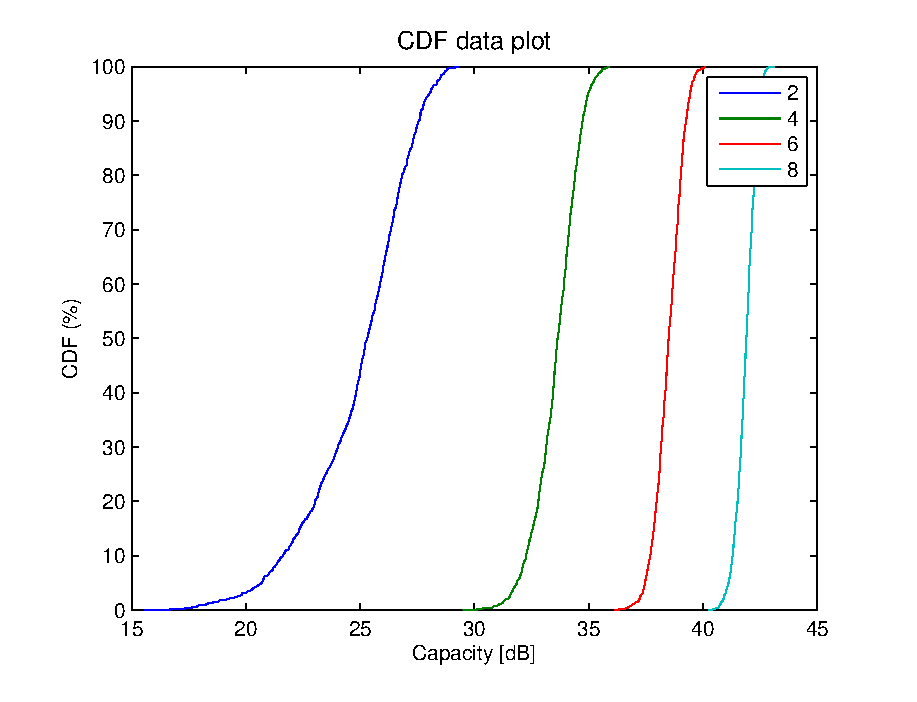
\includegraphics[width=10cm]{MIMO_capacity.eps}
  \caption{Capacity of a MIMO system using from 2 up to 8 antennas for 10dB SNR}
  \label{fig:MIMO_capacity}
\end{figure}
As it can be seen, using higher order MIMO implies an increase in capacity. By doubling the number of antennas from 2 to 4 and from 4 to 8, there is also an increase in capacity with 10 dB. \\

The capacity for low SNR values(5 dB) is shown in \figref{fig:MIMO_capacity_low_SNR} and for high SNR values in \figref{fig:MIMO_capacity_high_SNR}. It can be seen from the two figures that the ergodic capacity of the system is higher for high SNR values. The \SI{10}{\percent} outage capacity means that \SI{90}{\percent} of the channel realizations have guaranteed data capacity, which can also be depicted in the two CDF plots.
\begin{figure}[!h]
  \centering
  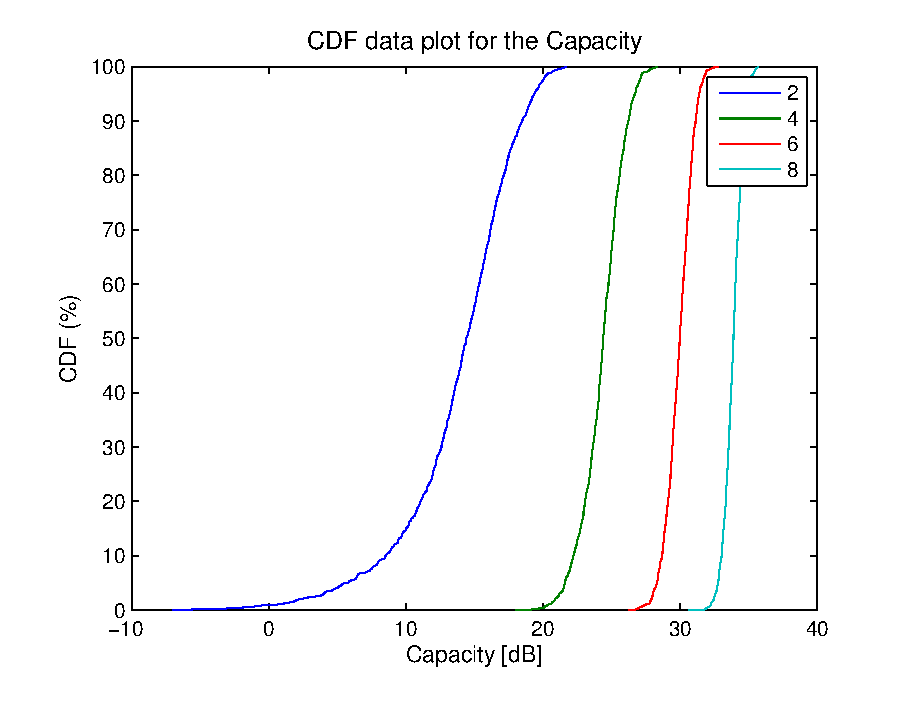
\includegraphics[width=10cm]{MIMO_capacity_low_SNR.eps}
  \caption{Capacity of a MIMO system using from 2 up to 8 antennas for 5dB SNR}
  \label{fig:MIMO_capacity_low_SNR}
\end{figure}
\begin{figure}[!h]
  \centering
  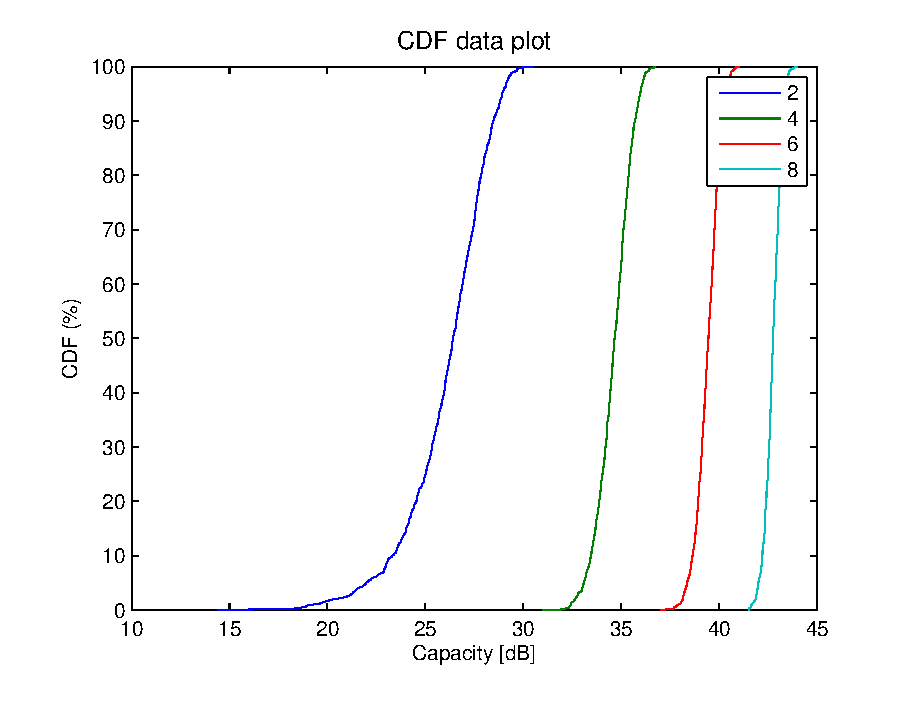
\includegraphics[width=10cm]{MIMO_capacity_high_SNR.eps}
  \caption{Capacity of a MIMO system using from 2 up to 8 antennas for 25dB SNR}
  \label{fig:MIMO_capacity_high_SNR}
\end{figure}

%The channel capacity is also higly related to the correlation between transmit and receive antennas. The capacity is reduced as the correlation becomes higher.
%The maximum outage capacity can be defined as the maximum rate that can be maintained in all channel states with some probability of outage (no data transmission).
